\documentclass[UTF8,a4paper,zihao=-4,fontset=mac]{ctexart}
\usepackage[margin=2.35cm]{geometry}
\usepackage{amsmath,amssymb,amsthm,booktabs,array,graphicx,float,caption}
\usepackage{xcolor,hyperref,fancyhdr,enumitem,tikz}
\usetikzlibrary{positioning,arrows.meta,fit}
\setmainfont{Times New Roman}
\setlength{\parindent}{2em}
\setlength{\parskip}{0pt}
\linespread{1.15}
\setlist{nosep,leftmargin=2em}
\captionsetup{font=small,labelsep=quad}
\renewcommand{\topfraction}{0.9}
\renewcommand{\textfraction}{0.08}
\renewcommand{\floatpagefraction}{0.85}
\hypersetup{hidelinks}
\pagestyle{fancy}\fancyhf{}\fancyfoot[C]{\thepage}
\renewcommand{\headrulewidth}{0pt}
\newcommand{\pos}[1]{\left(#1\right)_+}
\newcommand{\E}{\mathbb E}
\newcommand{\R}{\mathbb R}
\newtheorem{proposition}{命题}
\newtheorem{remark}{说明}
\title{基于跨日随机控制与价值反馈的微网购电和储能协同调度}
\author{}
\date{}

\begin{document}
\maketitle
\vspace{-2.1em}
\begin{abstract}
微网调度同时受到光伏和负荷预测误差、合同提前确定、紧急购电价格较高以及储能跨日库存价值的影响。若每天强制电池回到同一库存，会截断库存的跨日经济价值；若用未来真实量替代尚未发布的信息，又会高估策略收益。本文把四问统一为一个带合同、库存和实时反馈的随机动态系统，构造“成熟历史残差场景—因果合同规划—凸 Markov 动态规划反馈—滚动重规划—真实闭环结算”的控制框架。

针对问题一，建立连续线性规划并证明在非负电价、允许弃电的条件下，同时充放电可以结构性消除；指定日全天购电量为 $59482.70$ kWh，购电费为 $35126.95$ 元。针对问题二，在中间午夜连续、真实年末统一为 $6000$ kWh 的条件下，采用历史成熟残差场景和实时库存价值反馈，334 日费用为 $13844170.06$ 元，较每日闭合基线降低 $2.3818\%$。针对问题三，在不改变合同调整权限的情况下分离预报信息与合同执行，全年费用为 $13461842.35$ 元；相对只保留零点预报，完整的 $0$、$6$、$12$、$18$ 时预报使闭环费用减少 $316849.08$ 元，其中删除 $12$ 时预报造成的增量最大。针对问题四，净需求与价格共同不确定时，问题四-2和问题四-3费用分别为 $14654611.38$ 元和 $14252083.03$ 元，相对同口径每日闭合基线分别降低 $2.3716\%$ 和 $2.9260\%$。

在同一真实首末库存下，逐日账单的 $3$、$7$、$14$ 日移动块 bootstrap 区间均为正；月度总节省在 $11$ 个月均为正。但本文结果仅针对给定年度数据、披露规则和结算口径；完美信息线性规划只是乐观参照，不能把其与实际策略的差距全部解释为算法损失，也不据此声称得到原随机控制问题的全局最优解。
\end{abstract}
\noindent\textbf{关键词：}跨日储能；随机规划；因果合同；动态规划；滚动优化；微网经济调度

\section{问题重述与总体思路}
题目中的四个问题并非四个互不相关的静态优化问题，而是同一微网动态系统在不同信息权限下的特例；这种将储能、预测和滚动控制统一处理的视角与微网模型预测控制和储能套利研究相一致\cite{microgrid,storage}。问题一给出确定的负荷、光伏和电价，考察单日电池套利与购电安排；问题二要求在实际净需求实现前签订合同，偏差以高价紧急购电补足；问题三增加 $0$、$6$、$12$、$18$ 时发布的未来光伏预报和日内调约；问题四进一步使电价随时间变化，库存同时面对供需不确定性和价格不确定性。

本文的核心判断是：合同和电池动作不应使用同一信息集合。合同必须在当前净需求实现前决定，而电池可以在当前净需求被观测后反馈控制；与此同时，库存不应在每个午夜被人为清零，而应作为跨日状态连续传递。由此形成如下闭环：
\begin{equation}
\text{合法信息}\ \longrightarrow\ \text{成熟历史场景}\ \longrightarrow\ \text{因果合同规划}\ \longrightarrow\ \text{实时库存反馈}\ \longrightarrow\ \text{真实账单}.
\end{equation}

\begin{figure}[H]
\centering
\begin{tikzpicture}[x=1cm,y=1cm,>=Latex,font=\small]
  \node[draw,rounded corners,fill=blue!7,minimum width=2.35cm,minimum height=0.72cm] (obs) at (0,0) {历史观测与预报};
  \node[draw,rounded corners,fill=green!8,minimum width=2.35cm,minimum height=0.72cm] (scen) at (3.1,0) {成熟残差场景};
  \node[draw,rounded corners,fill=orange!12,minimum width=2.35cm,minimum height=0.72cm] (contract) at (6.2,0) {合同规划};
  \node[draw,rounded corners,fill=purple!9,minimum width=2.35cm,minimum height=0.72cm] (dp) at (9.3,0) {Markov 价值反馈};
  \node[draw,rounded corners,fill=red!8,minimum width=2.35cm,minimum height=0.72cm] (bill) at (12.4,0) {执行与结算};
  \draw[->] (obs)--(scen); \draw[->] (scen)--(contract); \draw[->] (contract)--(dp); \draw[->] (dp)--(bill);
  \draw[->,dashed] (bill.south) .. controls +(0,-1.1) and +(0,-1.1) .. node[below]{库存与已实现信息滚动更新} (obs.south);
  \node[align=center] at (1.55,-1.9) {只使用已知信息};
  \node[align=center] at (4.65,-1.9) {历史目标满足成熟性};
  \node[align=center] at (7.75,-1.9) {合同先于当前实现};
  \node[align=center] at (10.85,-1.9) {动作可看见当前净需求};
\end{tikzpicture}
\caption{跨日库存—因果合同—实时反馈的闭环结构。}
\end{figure}

\section{假设、信息结构与符号}
\subsection{建模假设}
\begin{enumerate}
  \item 电池额定容量为 $12000$ kWh，库存范围为 $[1200,10800]$ kWh，初始库存为 $6000$ kWh；充、放电单向效率均为 $\eta=0.9$，功率上限为 $5000$ kW。
  \item 每个控制时段为 $10$ min，输入功率按时段平均值积分；不售电，富余电允许弃置；题面未给出的自放电、老化、外网容量和线损参数不另行添加。
  \item 合同量、充放电量和紧急购电均采用母线侧电量口径。$q_t$ 表示日初原合同，$r_t$ 表示交付前最后生效的合同，二者不相加。
  \item 当前净需求在电池动作前可观测；未来真实负荷、光伏和电价不可提前使用。浮动电价在当前动作后进入结算，控制器只使用当时合法的预测或条件价格。
  \item 问题二至四的正式评价区间为 $2025$ 年 $2$ 月 $1$ 日至 $12$ 月 $31$ 日，共 $334$ 日；期初和真实评价终点库存均固定为 $6000$ kWh，中间午夜库存连续，不重置。
\end{enumerate}

\subsection{信息时序}
令 $a$ 为当前规划原点，$\mathcal F_t^-$ 为交付前已知信息，包含此前真实观测、已发布预报、现有合同和库存；当前净需求揭示后的动作信息为
\begin{equation}
\mathcal F_t=\mathcal F_t^-\vee\sigma(n_t).
\end{equation}
合同决策对 $\mathcal F_t^-$ 可测，电池动作对 $\mathcal F_t$ 可测，当前真实价格不属于动作决策信息。问题三的预报发布和调约权限严格分开：删去一批预报的消融实验仍保留四个调约节点，只改变可用信息。

\begin{figure}[H]
\centering
\begin{tabular}{c|c|c|c|c}
\toprule
节点 & 已发布预报 & 已观测净需求 & 可调整合同 & 可执行动作\\\midrule
$0$ 时 & 零点预报 & 截至上一时段 & 签订原合同 & 当前时段动作\\
$6$ 时 & 零点、六点 & 截至 $6$ 时前 & 修改未交付部分 & 修改后反馈\\
$12$ 时 & 再加十二点 & 截至 $12$ 时前 & 修改未交付部分 & 修改后反馈\\
$18$ 时 & 再加十八点 & 截至 $18$ 时前 & 修改未交付部分 & 修改后反馈\\
午夜 & 下一日信息起点 & 当日全部实现 & 新日合同 & 库存连续传递\\
\bottomrule
\end{tabular}
\caption{合法信息与动作权限。真实价格只在实际交付后进入账单。}
\end{figure}

\subsection{符号表}
\begin{table}[H]\centering\small
\caption{主要符号及其物理口径}
\begin{tabular}{lll}\toprule
符号 & 含义 & 单位\\\midrule
$t,d,\Delta$ & 全局时段、日期、时段长度 & --、--、$1/6$ h\\
$L_t,P_t,n_t$ & 负荷、光伏、净需求 & kW、kW、kWh\\
$q_t,r_t$ & 原合同、当前生效合同 & kWh\\
$c_t,d_t,e_t,s_t$ & 母线充电、放电、紧急购电、弃电 & kWh\\
$E_t$ & 电池内部储能 & kWh\\
$p_t,\widehat p_t$ & 实际结算价、合法价格预测 & 元/kWh\\
$\omega_s,\mathcal C_{t,k},V_{t,k}$ & 场景概率、Markov 状态组、库存值函数 & --\\
\bottomrule\end{tabular}
\end{table}

\section{问题一：确定性线性规划}
净需求由
\begin{equation}
n_t=\frac{L_t-P_t}{6}
\end{equation}
给出。能量平衡、库存递推和边界为
\begin{align}
r_t+e_t+d_t-c_t-s_t&=n_t,\\
E_{t+1}&=E_t+\eta c_t-d_t/\eta,\\
1200\le E_t&\le10800,\qquad 0\le c_t,d_t\le M,\quad M=5000/6.
\end{align}
问题一中 $r_t=q_t$，并要求 $E_0=E_{144}=6000$。目标为
\begin{equation}
\min J_1=\sum_{t=0}^{143}p_t(q_t+5e_t).
\end{equation}

\begin{proposition}[同时充放电的结构性消除]
在价格非负、富余电可免费弃置且不存在循环奖励的条件下，存在一个最优解满足 $c_td_t=0$。
\end{proposition}
\begin{proof}
令 $\Delta=E_{t+1}-E_t$。若 $\Delta\ge0$，可取 $c_t=\Delta/\eta,d_t=0$；若 $\Delta<0$，可取 $c_t=0,d_t=-\eta\Delta$。任意同时充放电的动作在保持 $\Delta$ 不变时会增加母线侧净耗电，富余部分又可被弃置，因此把循环量移除不会增加合同购电或紧急购电费用，也不改变下一库存。逐时替换即可得到不同时充放电的最优解。
\end{proof}

问题一结果见表~\ref{tab:q1}. 线性规划目标、约束残差和独立对偶证书的最大差异均小于 $10^{-10}$ 元量级；该结论只证明确定性 LP 的正确性，不延伸为随机问题的全局最优性。
\begin{table}[H]\centering\small
\caption{问题一确定性结果}\label{tab:q1}
\begin{tabular}{l r}
\toprule
指标 & 数值\\\midrule
全天购电量 / kWh & 59482.6990\\
全天购电费 / 元 & 35126.9486\\
母线侧总充电量 / kWh & 20740.6661\\
母线侧总放电量 / kWh & 16799.9396\\
库存最小—最大 / kWh & $1200.0000$—$10800.0000$\\
首、末库存 / kWh & $6000.0000$、$6000.0000$\\
\bottomrule
\end{tabular}
\end{table}

\begin{table}[H]\centering\small
\caption{问题一指定时段购电与分段充放电}
\begin{tabular}{c|r@{\quad}c|r r}
\toprule
时段 & 购电量/kWh & 分段 & 充电量/kWh & 放电量/kWh\\\midrule
10:00--10:10 & 0.0000 & 00:00--04:00 & 4500.0000 & 0.0000\\
12:00--12:10 & 480.4124 & 04:00--08:00 & 833.3333 & 6365.8412\\
14:00--14:10 & 0.0000 & 08:00--12:00 & 4787.9643 & 1702.9970\\
16:00--16:10 & 445.4317 & 12:00--16:00 & 5286.0352 & 91.1014\\
18:00--18:10 & 531.8940 & 16:00--20:00 & 0.0000 & 5780.1319\\
20:00--20:10 & 0.0000 & 20:00--24:00 & 5333.3333 & 2859.8681\\
\bottomrule
\end{tabular}
\end{table}

\section{问题二至四：统一随机动态模型}
\subsection{闭环账单与跨日库存}
允许调约时，题面计费口径可写为
\begin{equation}\label{eq:bill}
J=\sum_t p_t\left[q_t+1.5\pos{r_t-q_t}-0.5\pos{q_t-r_t}+5e_t\right]
=\sum_t p_t\left[r_t+0.5|r_t-q_t|+5e_t\right].
\end{equation}
问题二和问题四-2令 $r_t=q_t$；问题三和问题四-3只在已发布节点调整未交付合同。每个午夜满足
\begin{equation}
E_{d+1,0}=E_{d,144},
\end{equation}
只有真正评价期末要求 $E_{T_\star}=6000$。每日闭合基线额外强制所有午夜为 $6000$，因而是可比较但更强的库存约束。

\subsection{成熟历史残差场景}
在当前规划时刻 $a$ 生成长度为 $T$ 的历史残差块时，候选起点 $h$ 必须满足。该有限样本场景近似属于随机规划中的样本平均与场景缩减范畴\cite{shapiro,kl,scenario}，但本文额外施加了信息成熟性约束。
\begin{equation}
\mathcal H_a=\{h:h+T\le a,\ h\equiv a\pmod {144}\}.
\end{equation}
不满足该条件的块，即使其覆盖的未来数据已经存放在本地，也不能进入当前场景集合。它保证历史目标整体已在当前决策前真实发生，不把尚未揭示的预报或真实量泄漏到合同规划。对合法残差块按当前已知状态计算距离并加权，随后以加权前向选择保留 $S=7$ 条代表轨迹。

\subsection{因果仿射合同规划}
合同在当前净需求实现前决定，未来合同只能依赖此前已经揭示的历史特征。对场景 $s$，用中心化误差特征 $\phi$ 表示因果扰动反馈。这种决策规则可视为不确定线性规划中的可调策略参数化\cite{adjustable}：
\begin{align}
q_t^s&=\bar q_t+K^q_{\rho_q(t)}\phi^s_{\rho_q(t)},\\
r_t^s&=\bar r_t+K^r_{\rho_r(t)}\phi^s_{\rho_r(t)}.
\end{align}
其中 $\rho_q(t)$ 是日初合同节点，$\rho_r(t)$ 是题面允许的 $6$ 小时节点；在不允许调约的时段施加 $r_t=q_t$。该策略类不是对所有扰动路径的鲁棒保证，而是在合法经验场景上规划、由物理执行器在真实轨迹上投影和结算的因果决策规则。

\subsection{Markov 实时价值反馈}
库存 $E$ 表示尚可使用的电能资源，当前净需求状态反映近期供需压力。将场景净需求按三分位划分为 $k\in\{1,2,3\}$，以场景相邻时段标签和伪计数得到转移矩阵 $P_{t,k\ell}$。组内价格采用合法场景条件均值 $\bar p_{t,k}$。这是对动态规划和滚动控制中状态—价值递推思想的有限状态近似\cite{bertsekas,rawlings}。令
\begin{equation}
g(\Delta E)=\max\{\eta\Delta E,\Delta E/\eta\}
\end{equation}
为实现库存变化 $\Delta E=E'-E$ 时的最小母线侧净耗电，库存可行域为
\begin{equation}
\mathcal E(E)=[\max\{1200,E-M/\eta\},\min\{10800,E+\eta M\}].
\end{equation}
固定合同后，普通合同费用与电池动作无关；实时反馈的近似 Bellman 递推为
\begin{equation}\label{eq:bellman}
V_{t,k}(E)=\sum_{s\in\mathcal C_{t,k}}\omega_{s|k}
\min_{E'\in\mathcal E(E)}\left\{5\bar p_{t,k}\pos{n_t^s-r_t+g(E'-E)}+\sum_{\ell}P_{t,k\ell}V_{t+1,\ell}(E')\right\}.
\end{equation}
实际执行时，先观测当前 $n_t$，再选择对应状态组和连续库存动作；当前真实价格不提前进入控制。库存值函数在 $321$ 个节点上以凸分段线性方式存储。

式~\eqref{eq:bellman} 的凸性来自两个事实：即时紧急购电成本是库存变化的凸分段线性函数；未来值函数与其在库存转移约束下做下确界卷积仍保持凸性。因此储能动作可以连续优化，而不必用充放电互斥二进制变量。Markov 三状态是有限历史样本下对持续性的一阶压缩，不声称是完整随机过程的充分统计量。

\subsection{问题三预报与问题四价格}
问题三只在预报实际发布后使用相应光伏序列；历史预测和官方预报按当前可见范围融合，未来正式更新不能回填到此前合同。预报消融保持 $0,6,12,18$ 时的合同调整权限不变，只删除指定发布的信息。这里将预测信息转化为合同与动作，是预测到决策映射意义上的处方式分析\cite{prescriptive}。

问题四把净需求残差与价格残差作为同一历史块中的联合外生过程，保留两者相关性。控制器使用历史条件价格或已发布的价格预测，真实价格仅进入式~\eqref{eq:bill} 的结算。这样，价格预测误差不会被错误地当作已知未来价格。

\subsection{滚动执行与辅助 SDDP}
每个合法合同节点重新规划，随后每个 $10$ min 按最新观测执行；账单由真实 $q,r,e,p$ 逐时重算。SDDP 只作为同一实时反馈结构下的继续价值备选，其思想源于多阶段随机规划的切割近似\cite{sddp}：其辅助模型按月训练、时间聚合并假定阶段独立噪声，不能替代原始问题的完整多阶段随机最优值。最终采用简单线性库存末值，是因为开发期和全年闭环账单中，SDDP 末值没有降低真实费用；模型选择依据真实闭环成本而非算法复杂度。

\section{实验设计与结果}
\subsection{评价口径与数值验证}
冻结基线的正式评价采用同一 $334$ 日真实序列、相同初末库存、相同物理约束和相同结算器。除特别注明外，表中“基线”均指每日午夜闭合的 Markov 反馈基线；“主策略”指中间午夜连续、年末固定 $6000$ 的 Markov 反馈。所有候选的母线平衡、库存递推、容量、功率、单向充放、午夜连续、合同发布权限和账单均由独立程序复核。冻结计算的独立生产审计覆盖 $36$ 组轨迹，未关闭问题为 $0$ 项；其范围是数值和执行正确性，不是原随机问题全局最优性证明。

\begin{table}[H]\centering\small
\caption{334 日同真实首末库存的主结果}
\begin{tabular}{l r r r r}
\toprule
问题 & 每日闭合基线/元 & 主策略/元 & 节省/元 & 节省率\\\midrule
问题二 & 14181955.66 & 13844170.06 & 337785.60 & 2.3818\%\\
问题三 & 13828014.10 & 13461842.35 & 366171.75 & 2.6480\%\\
问题四-2 & 15010601.46 & 14654611.38 & 355990.08 & 2.3716\%\\
问题四-3 & 14681668.45 & 14252083.03 & 429585.42 & 2.9260\%\\
\bottomrule
\end{tabular}
\end{table}

主策略的年末固定库存并非强制每个午夜闭合。若将年末放开，四个主策略费用分别为 $13841680.52$、$13459169.01$、$14652127.40$、$14249362.50$ 元；与固定年末相比的差额仅为末端条件敏感性，不能全部解释为跨日库存收益。

\subsection{控制变量链：库存连续、合同规划与实时反馈}
为分离机制，先在相同真实首末库存下比较每日闭合仿射执行与跨日仿射执行，再比较同一跨日合同规划下的仿射反馈与 Markov 反馈。前一对照只改变中间午夜是否闭合，后一对照主要检验实时价值反馈。
\begin{table}[H]\centering\small
\caption{同终点的跨日库存与反馈对照}
\begin{tabular}{l r r r|r r}
\toprule
问题 & 闭合仿射 & 跨日仿射 & 跨日节省 & 跨日 Markov & Markov 相对仿射\\\midrule
问题二 & 14806348.92 & 14579795.71 & 226553.21 & 13844170.06 & 735625.65\\
问题三 & 14351793.81 & 14047627.45 & 304166.35 & 13461842.35 & 585785.10\\
问题四-2 & 15690288.96 & 15417329.12 & 272959.85 & 14654611.38 & 762717.74\\
问题四-3 & 15181643.82 & 14848008.86 & 333634.96 & 14252083.03 & 595925.84\\
\bottomrule
\end{tabular}
\end{table}
这一组对照支持两点：在同一仿射策略类、相同真实终点和相同信息权限下，取消中间午夜闭合具有实际经济价值；在此基础上，Markov 反馈进一步利用了“当前库存—当前供需状态”的价值关系。由于两条闭环轨迹的库存会影响后续合同，表中不能将每一项差额理解为彼此完全独立的可加贡献。

\begin{figure}[H]\centering
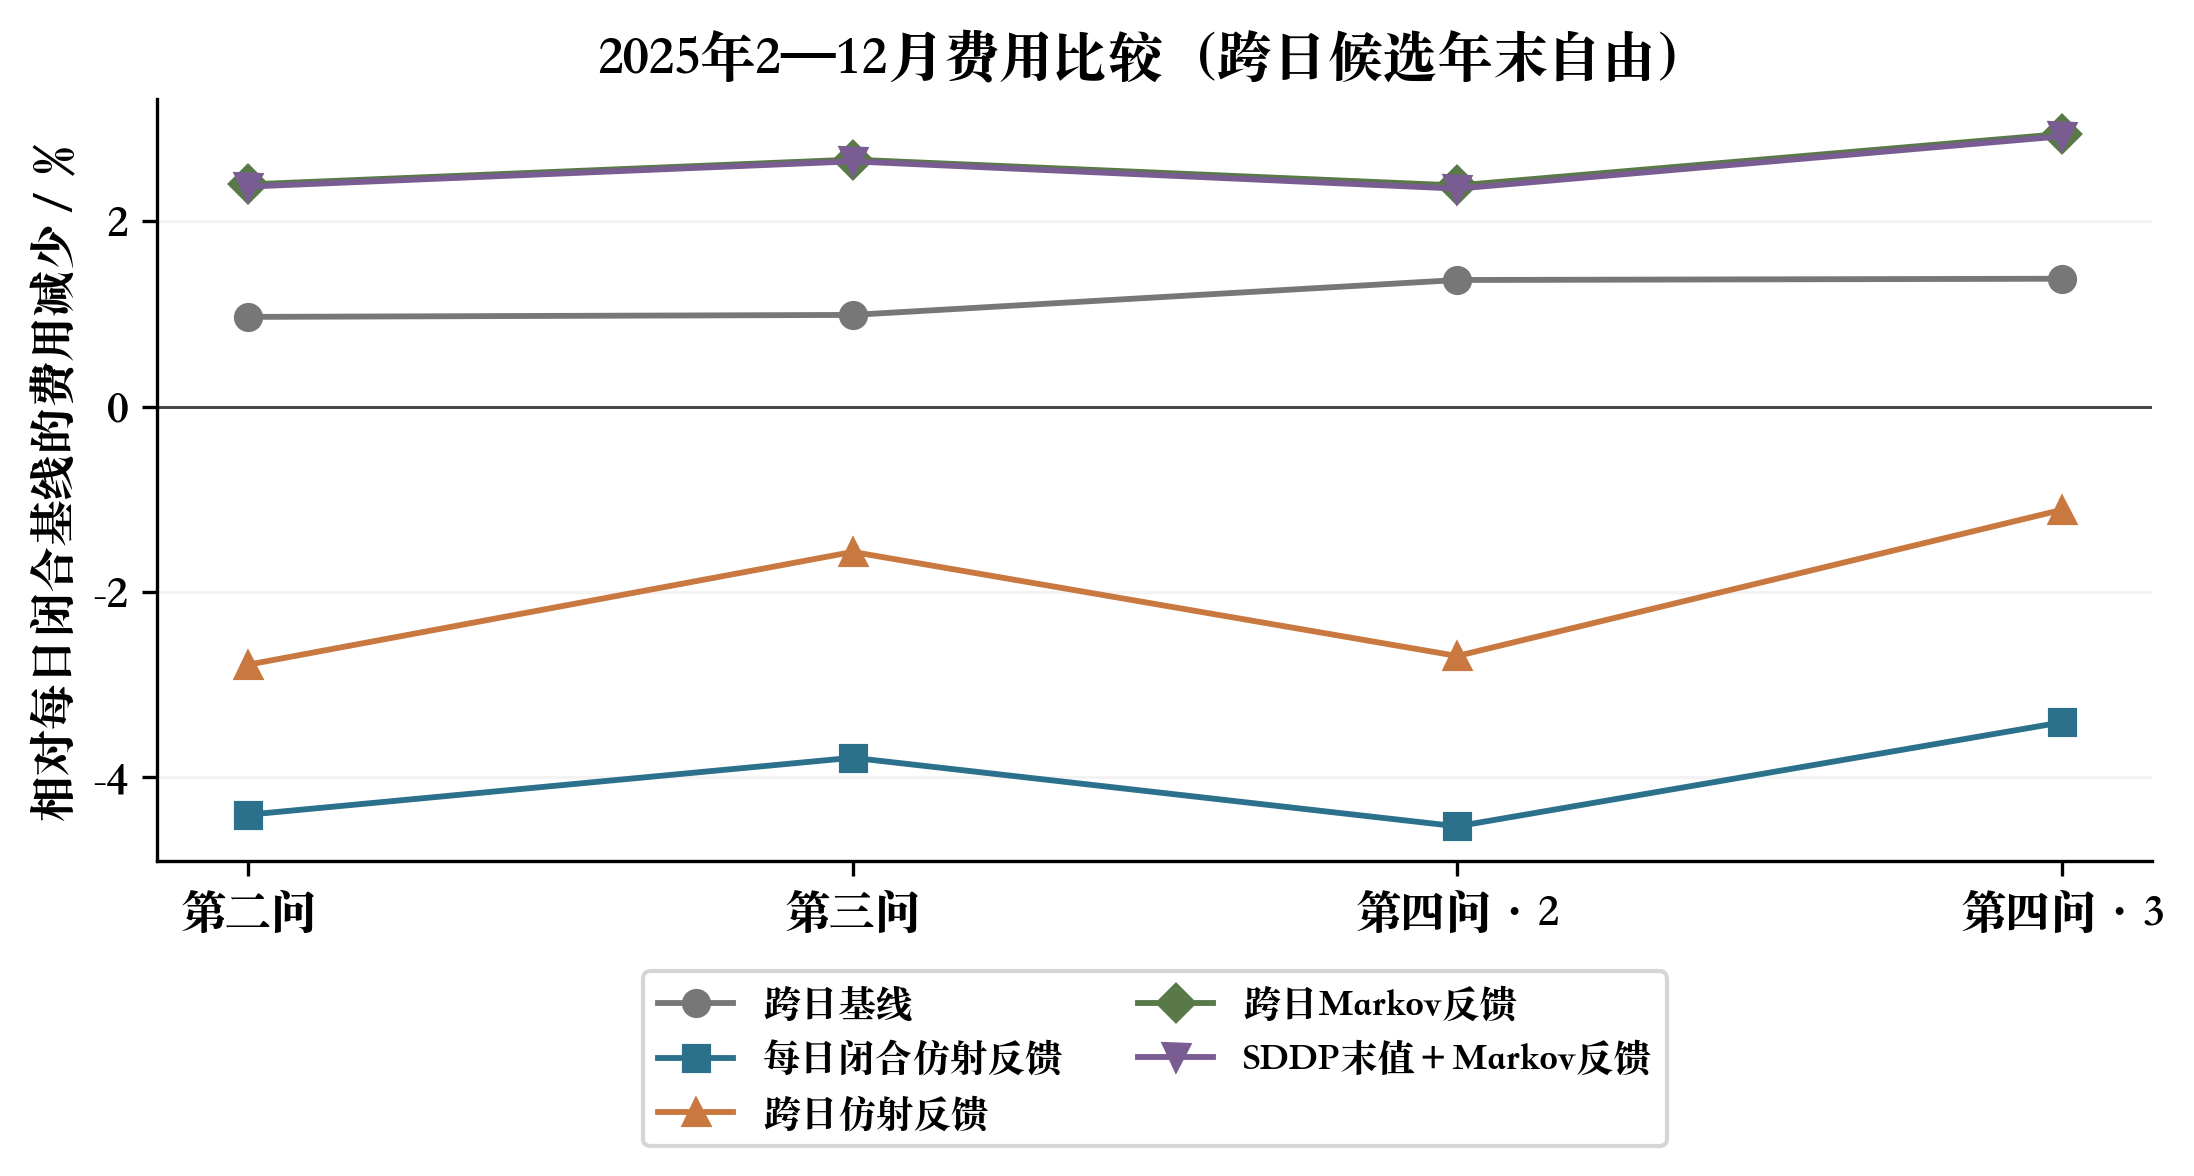
\includegraphics[width=.84\linewidth]{../baseline_frozen/figures/年度方法比较.png}
\caption{冻结基线中的年度方法比较。自由年末与固定年末结果分开解释。}
\end{figure}

\subsection{问题三：预报信息价值}
保持四个合同调整节点不变，只移除指定光伏预报，使用同一初末库存和同一旧策略的固定终点后缀。完整预报主策略费用为 $13461842.35$ 元；删去某批预报后的费用增加见表~\ref{tab:forecast}。
\begin{table}[H]\centering\small
\caption{问题三正式预报发布的同终点消融}\label{tab:forecast}
\begin{tabular}{l r r r}
\toprule
保留信息 & 总费用/元 & 相对完整预报增量/元 & 增量率\\\midrule
完整 $0,6,12,18$ 时预报 & 13461842.35 & 0.00 & 0.0000\%\\
仅零点预报 & 13778691.44 & 316849.08 & 2.3537\%\\
去掉六点预报 & 13533796.50 & 71954.15 & 0.5345\%\\
去掉十二点预报 & 13641121.93 & 179279.58 & 1.3318\%\\
去掉十八点预报 & 13462799.98 & 957.63 & 0.0071\%\\
\bottomrule
\end{tabular}
\end{table}
在当前数据和策略下，十二点预报的信息敏感性最高，六点次之，十八点最低。该结果是固定策略的信息消融，不是所有可行策略下的严格信息价值；各批预报之间存在交互，不能将单独删除增量简单相加。

\begin{figure}[H]\centering
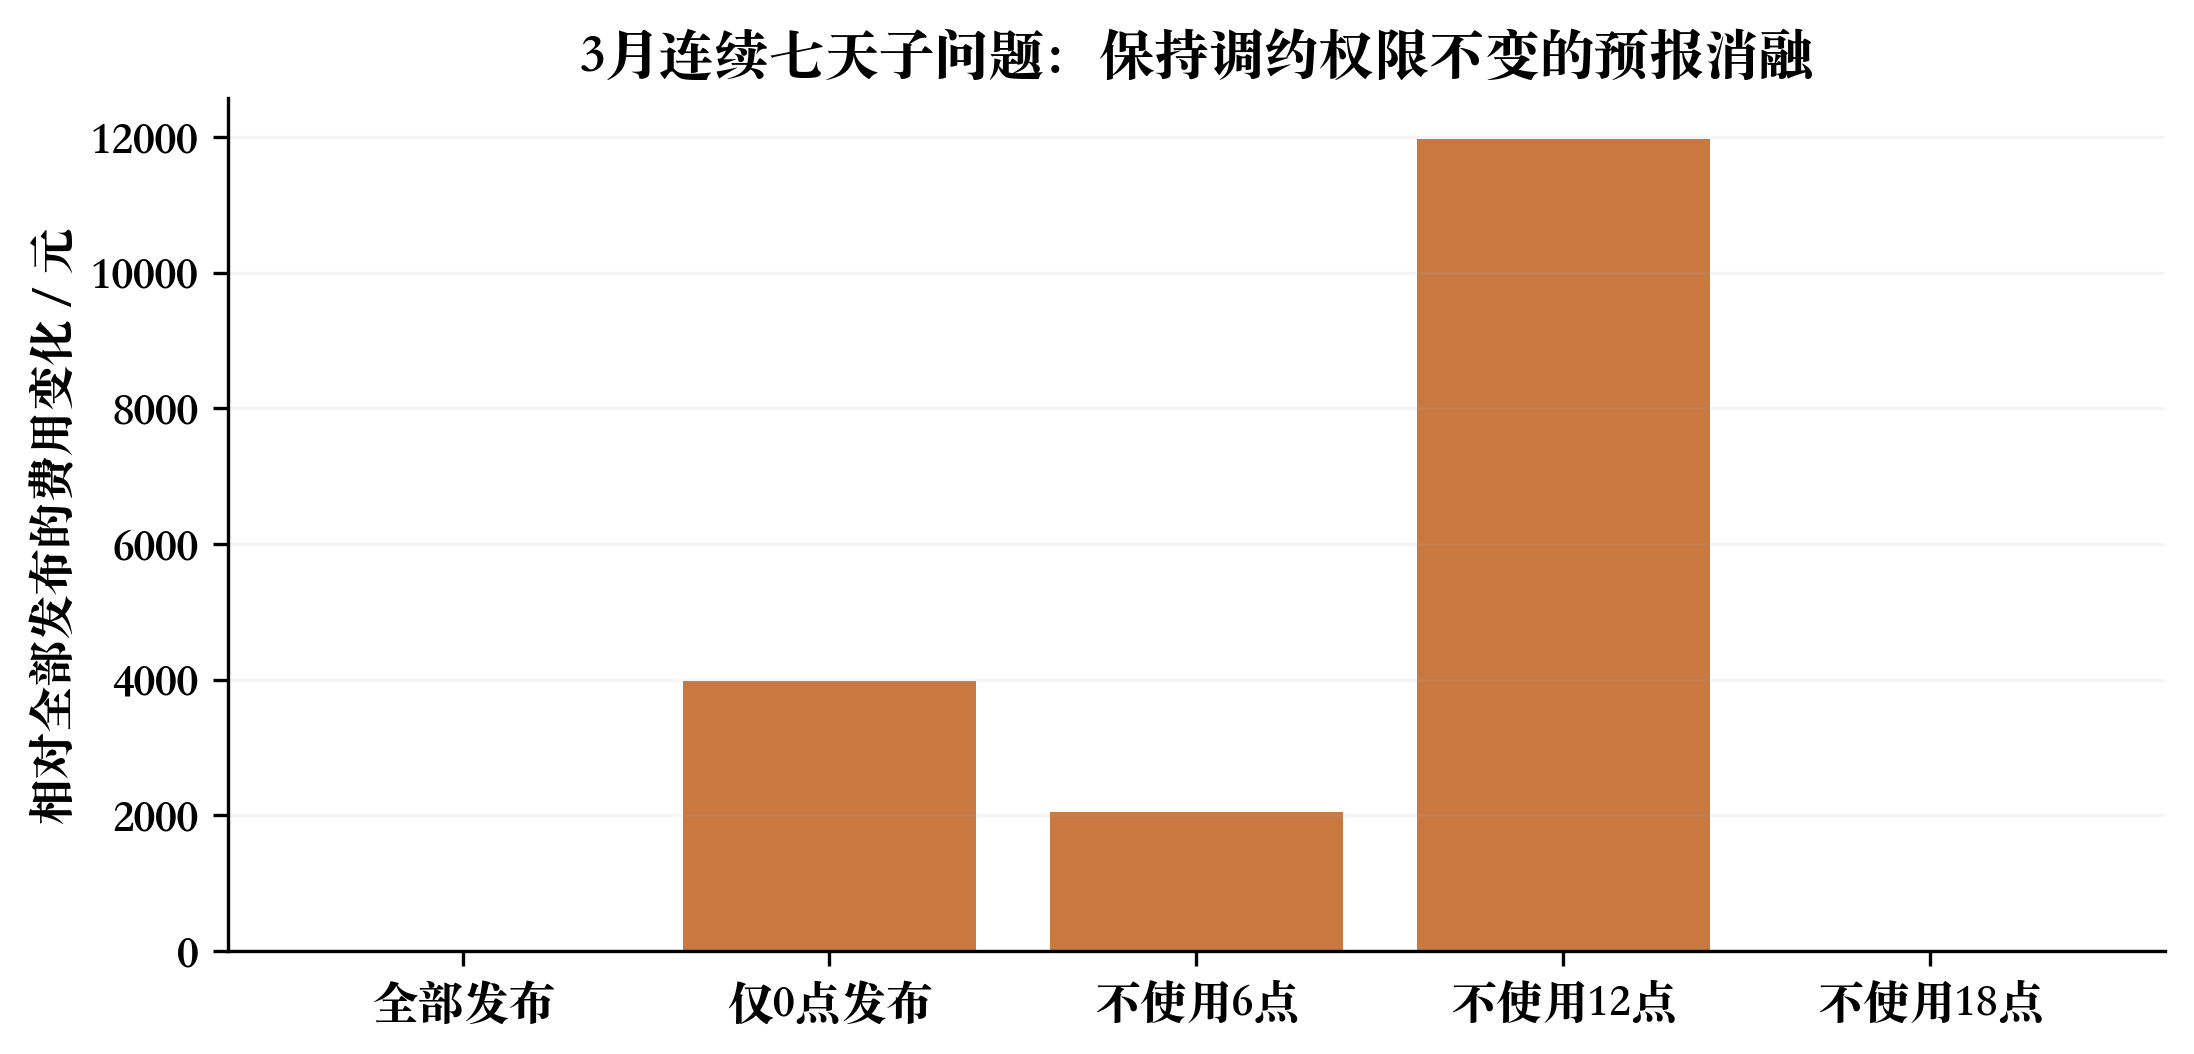
\includegraphics[width=.82\linewidth]{../baseline_frozen/figures/预报发布消融.png}
\caption{预报发布消融结果；权限保持不变，变化来自可用预报信息。}
\end{figure}

\subsection{问题四：时变电价}
问题四-2不允许日内调约，问题四-3允许在合法预报节点调约。两者均把价格与净需求放在同一历史场景中，并只在交付后用真实价格结算。相对每日闭合基线，允许调约的 Q4-3 节省率高于 Q4-2，但这不是把价格信息提前输入控制器的结果，而是合同权限和反馈的共同作用。

\begin{table}[H]\centering\small
\caption{主策略账单分解}
\begin{tabular}{l r r r r}
\toprule
问题 & 主策略总费用/元 & 紧急购电量/kWh & 弃电量/kWh & 日胜出数\\\midrule
问题二 & 13844170.06 & 151764.08 & 2336748.17 & 268\\
问题三 & 13461842.35 & 37821.57 & 1738320.52 & 284\\
问题四-2 & 14654611.38 & 139989.69 & 2373217.79 & 229\\
问题四-3 & 14252083.03 & 37930.27 & 1746588.10 & 241\\
\bottomrule
\end{tabular}
\end{table}
弃电是母线侧总富余弃置，可能含已购电能，不能直接称为光伏弃电率。费用目标是式~\eqref{eq:bill} 的总账单，合同某一分项增加并不必然表示策略变差。

\subsection{SDDP、参数敏感性与性能边界}
开发期的简单线性末值与 SDDP 末值 Markov 反馈费用分别为：问题二 $344539.23$ 与 $344539.23$ 元，问题三 $339412.44$ 与 $339437.66$ 元，问题四-2 $384378.44$ 与 $384378.40$ 元，问题四-3 两者相同至数值精度。全年采用 SDDP 末值后，费用分别比线性末值高 $3295.29$、$2581.53$、$5119.87$ 和 $3714.94$ 元。因此保留更简单的末值模型，并把 SDDP 作为辅助继续价值而非主角。

参数实验中，库存网格 $161/321/641$、场景数、前瞻长度和末值倍率均在固定的连续七日窗口上检查。参考配置费用为 $243002.90$ 元；$161$ 点和 $641$ 点分别为 $242988.81$ 和 $243028.94$ 元，网格加密未呈现单调的账单改善。该现象说明网格分辨率需作为数值稳定性参数而不是按年度费用挑选。

完美信息全时域 LP 的固定终点费用为：\\
固定电价 $12230383.65$ 元，时变电价 $12783021.74$ 元。它预先知道全部真实路径，是实际因果策略的乐观参考。

实际策略与该参考的差距同时包含未来信息价值、有限场景、Markov 近似、滚动合同策略类和数值尾值误差，不写成单一“算法最优性 gap”。

\begin{figure}[H]\centering
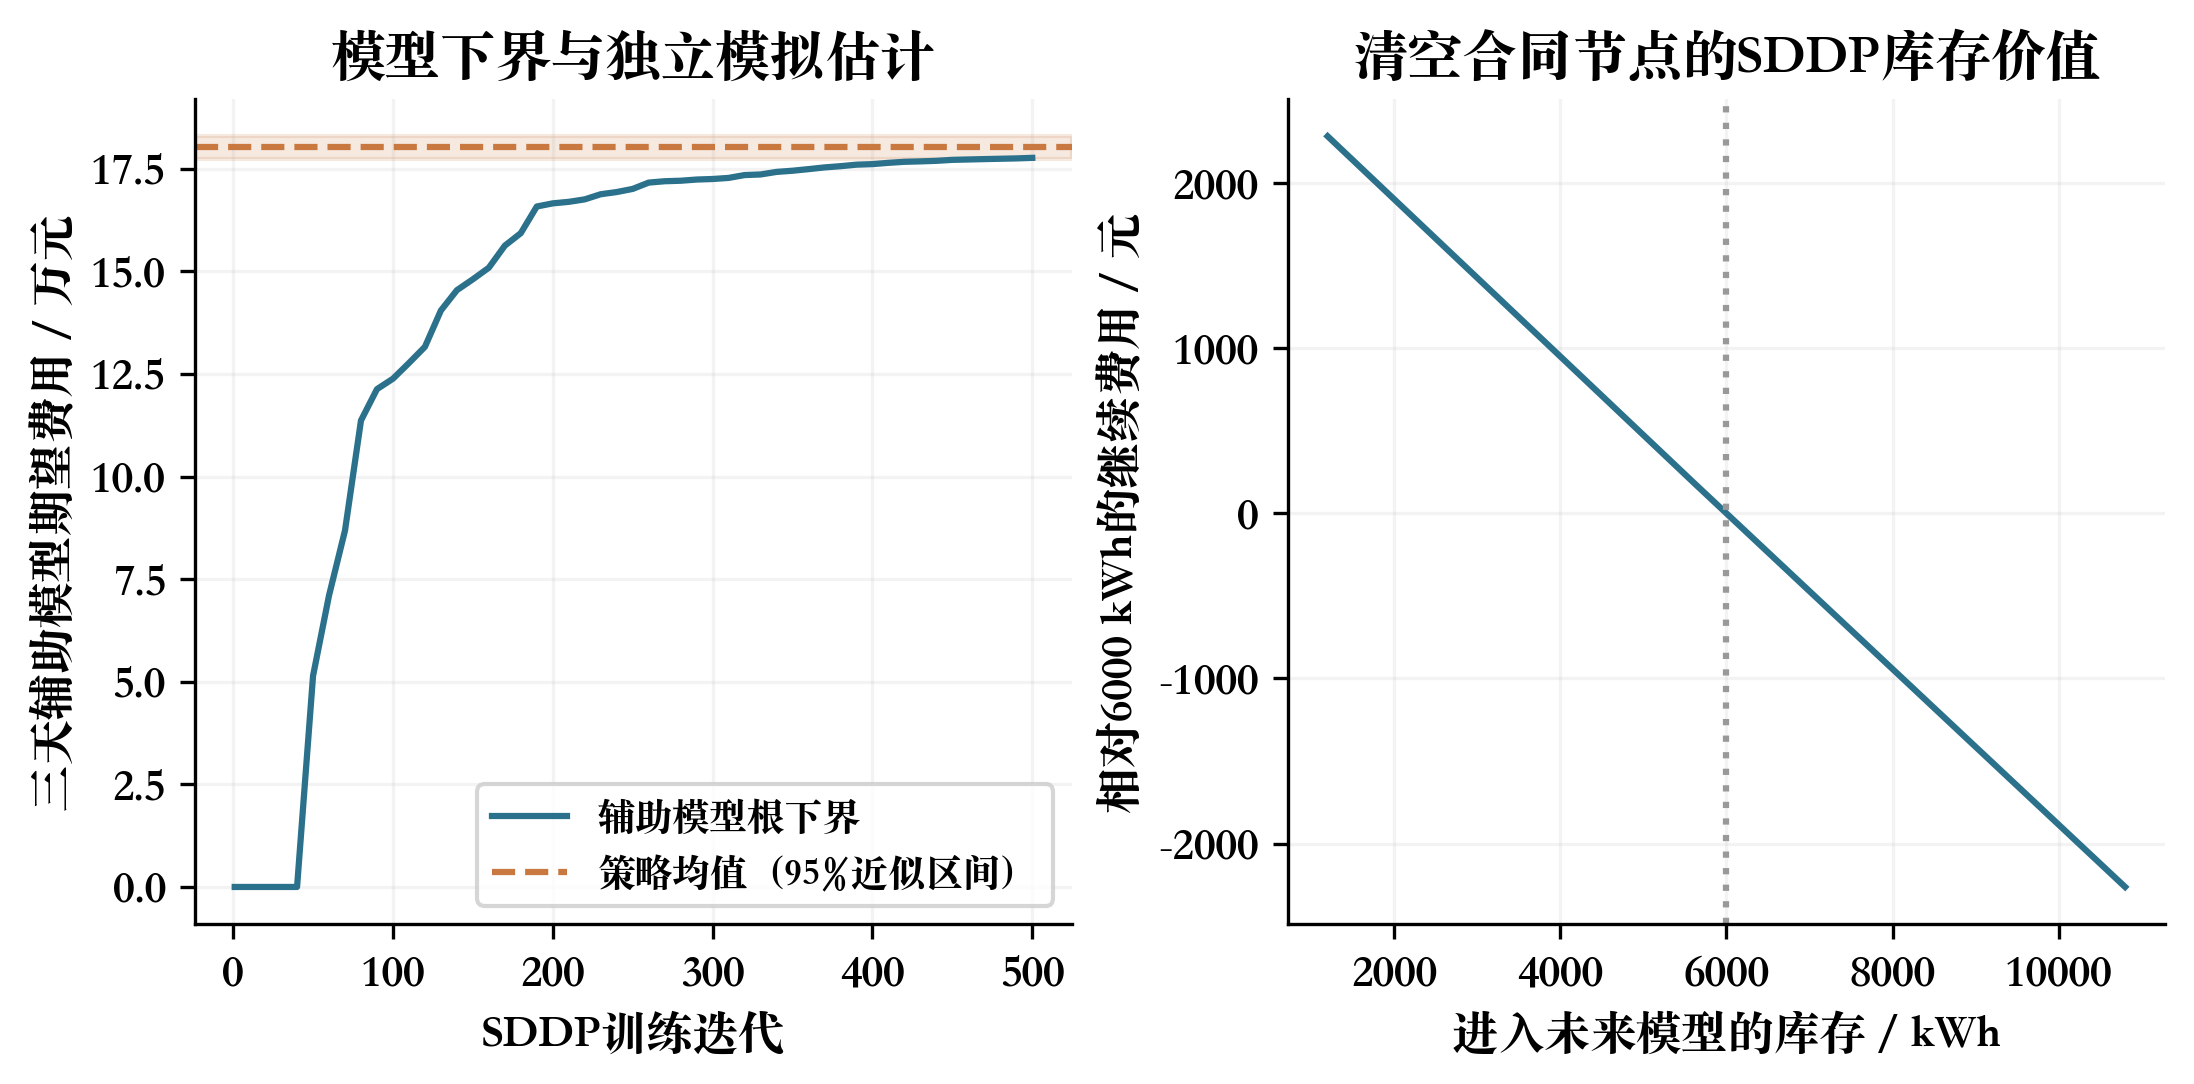
\includegraphics[width=.82\linewidth]{../baseline_frozen/figures/SDDP训练与库存价值.png}
\caption{辅助 SDDP 训练与库存价值诊断；其下界只针对辅助模型。}
\end{figure}

\subsection{时间稳定性：月份与移动块 bootstrap}
对每日配对节省 $\Delta_d=C_{d,\mathrm{baseline}}-C_{d,\mathrm{main}}$ 使用连续移动块重采样，块长取 $3$、$7$、$14$ 日，重复 $10000$ 次，随机种子为 $20260911$。这种保留时间相关性的重采样方法参照平稳观测的移动块 bootstrap\cite{kunsch}。表~\ref{tab:bootstrap} 报告主块长 $7$ 日的百分位 $95\%$ 区间；三个块长的区间均保持为正。该区间是单年度、带季节性的稳定性诊断，不是未来年度的分布无关置信保证。
\begin{table}[H]\centering\small
\caption{334 日配对节省与 7 日移动块区间}\label{tab:bootstrap}
\begin{tabular}{l r r r r}
\toprule
问题 & 累计节省/元 & 95\% 下限/元 & 95\% 上限/元 & 正/负日数\\\midrule
问题二 & 337785.60 & 276912.77 & 406410.55 & 268/66\\
问题三 & 366171.75 & 313534.58 & 417831.86 & 284/50\\
问题四-2 & 355990.08 & 295236.40 & 417351.79 & 229/105\\
问题四-3 & 429585.42 & 363235.99 & 495036.62 & 241/93\\
\bottomrule
\end{tabular}
\end{table}

月度累计节省在四个问题中均为正，因而为 $11/11$ 个月；但逐日仍存在负节省日，尤其是 Q4-2。冬季负荷高、夏季光伏和价格结构不同，月度绝对节省因此不应直接比较为同一物理机制的强弱。\(3\) 日和 \(14\) 日区间见附录表~\ref{tab:bootstrap-sensitivity}。

\section{模型评价、局限与可复现性}
\subsection{可信之处}
本文的主要可信度不来自算法名称，而来自约束与证据链：
\begin{enumerate}
  \item 合同、当前观测、预报发布和价格结算均有明确的信息截止；成熟块条件 $h+T\le a$ 阻断未来目标泄漏。
  \item 电池内部库存、母线充放电、合同购电、紧急购电和弃电分别建模，物理平衡与账单由真实闭环数组重新核算。
  \item 中间午夜连续、真正评价期末统一，且另报告自由年末敏感性；同终点仿射对照支持跨日库存本身的经济价值。
  \item 预报消融只删除信息，不删除合同调整权限；SDDP和完美信息 LP 均按其实际适用范围解释。
  \item 逐日配对采用时间相关的移动块 bootstrap，并保留负节省日，不以累计费用较低替代稳定性证据。
\end{enumerate}

\subsection{局限}
第一，数据只覆盖一个历史年度，不能据此证明跨年泛化、稳态平均成本或未来年度收益。第二，有限场景、三状态 Markov 和滚动合同是可计算近似，未获得原始随机控制问题的可识别因果下界。第三，SDDP按月时间聚合并阶段独立化，只是辅助末值；其训练下界不能直接解释为原题下界。第四，退购计费、当前净需求观测和价格披露是依据题面歧义作出的政策选择，改变这些口径需重新计算。第五，未引入题面未提供的电池退化、自放电和配网暂态参数。

\subsection{复现说明}
结果来源、逐时轨迹、独立审计和图表保存在本目录的冻结副本中。推荐入口为：
\begin{center}
\texttt{baseline\_frozen/模型与推导.md},\quad
\texttt{baseline\_frozen/建模计算交接.md},\quad
\texttt{baseline\_frozen/review/final-review.md}.
\end{center}
{\raggedright 论文数值证据由 \texttt{tools/build\_frozen\_paper\_evidence.py} 从冻结 NPZ/JSON 逐日重算，输出 \texttt{artifacts/frozen-paper-evidence.json}；所有纸面数值登记在 \texttt{artifacts/result-registry.json} 并映射到 \texttt{paper/result-claims.json}。复现时应先核对源文件哈希；任何源码或结果改变后，原独立审查哈希不自动延续。\par}

\section{结论}
针对微网购电与储能调控的四个问题，本文以跨日库存为状态主线，区分因果合同和实时电池动作的信息集合，用成熟历史残差生成有限场景，以凸 Markov 动态规划表达库存继续价值，并通过滚动重规划和真实账单闭环评价。确定性问题由连续 LP 正确求解；随机问题在同初末库存下，主策略相对每日闭合基线在四个设置分别降低 $2.3818\%$、$2.6480\%$、$2.3716\%$ 和 $2.9260\%$。同终点仿射对照说明跨日库存不是“自由年末消耗库存”造成的假象；预报消融说明正式更新的信息价值取决于更新时间和供需状态；价格不确定性则使库存价值随价格状态变化。

这些结论的适用范围严格限定在给定年度、信息披露和结算规则下。本文的贡献是建立一条可审计的因果控制与闭环验证链，而不是用复杂算法宣称全局最优。未来若取得独立年份、真实价格披露时间戳和电池退化参数，应在不改变评价口径的前提下进行外部验证。

\begin{thebibliography}{99}
\bibitem{shapiro}Shapiro A, Dentcheva D, Ruszczyński A. Lectures on Stochastic Programming: Modeling and Theory[M]. 2nd ed. Philadelphia: SIAM, 2014.
\bibitem{kl}Kleywegt A J, Shapiro A, Homem-de-Mello T. The sample average approximation method for stochastic discrete optimization[J]. SIAM Journal on Optimization, 2002, 12(2): 479--502.
\bibitem{birge}Birge J R, Louveaux F. Introduction to Stochastic Programming[M]. 2nd ed. New York: Springer, 2011.
\bibitem{rawlings}Rawlings J B, Mayne D Q, Diehl M M. Model Predictive Control: Theory, Computation, and Design[M]. 2nd ed. Madison: Nob Hill Publishing, 2017.
\bibitem{bertsekas}Bertsekas D P. Dynamic Programming and Optimal Control[M]. 4th ed. Belmont: Athena Scientific, 2017.
\bibitem{sddp}Pereira M V F, Pinto L M V G. Multi-stage stochastic optimization applied to energy planning[J]. Mathematical Programming, 1991, 52: 359--375.
\bibitem{adjustable}Ben-Tal A, Goryashko A, Guslitzer E, Nemirovski A. Adjustable robust solutions of uncertain linear programs[J]. Mathematical Programming, 2004, 99(2): 351--376.
\bibitem{scenario}Dupačová J, Gröwe-Kuska N, Römisch W. Scenario reduction in stochastic programming[J]. Mathematical Programming, 2003, 95(3): 493--511.
\bibitem{microgrid}Parisio A, Rikos E, Glielmo L. A model predictive control approach to microgrid operation optimization[J]. IEEE Transactions on Control Systems Technology, 2014, 22(5): 1813--1827.
\bibitem{storage}Sioshansi R, Denholm P, Jenkin T, Weiss J. Estimating the value of electricity storage in PJM: Arbitrage and regulation[J]. Energy Economics, 2009, 31(2): 269--277.
\bibitem{prescriptive}Bertsimas D, Kallus N. From predictive to prescriptive analytics[J]. Management Science, 2020, 66(3): 1025--1044.
\bibitem{kunsch}Künsch H R. The jackknife and the bootstrap for general stationary observations[J]. The Annals of Statistics, 1989, 17(3): 1217--1241.
\end{thebibliography}

\appendix
\section{算法伪代码}
\begin{enumerate}
  \item 在当前合法信息集内重建历史预测和误差账本，筛选满足 $h+T\le a$ 的成熟块。
  \item 对成熟块计算条件权重并缩减至 $7$ 条代表场景；在合同节点求解因果仿射规划。
  \item 用三状态 Markov 转移和库存凸值函数反向递推；观测当前净需求后求连续库存动作。
  \item 将动作投影至库存、功率和真实终点可达域，计算紧急购电与弃电；推进到下一 $10$ min。
  \item 在 $0,6,12,18$ 时只使用已发布预报修订未交付合同；每日结束继承库存，年末检查 $6000$ kWh。
  \item 用真实价格、最终合同和紧急购电逐时重算账单；再输出逐日费用与审计字段。
\end{enumerate}

\section{移动块敏感性}
\begin{table}[H]\centering\small
\caption{3、7、14 日移动块 bootstrap 区间（元）}\label{tab:bootstrap-sensitivity}
\begin{tabular}{l r@{\quad}r@{\quad}r}
\toprule
问题 & 3 日区间 & 7 日区间 & 14 日区间\\\midrule
问题二 & $[272298.80,410754.02]$ & $[276912.77,406410.55]$ & $[273801.64,406726.42]$\\
问题三 & $[313757.13,417129.63]$ & $[313534.58,417831.86]$ & $[304410.63,429506.28]$\\
问题四-2 & $[290749.29,423403.68]$ & $[295236.40,417351.79]$ & $[287021.39,429369.34]$\\
问题四-3 & $[370490.25,490203.33]$ & $[363235.99,495036.62]$ & $[351137.73,509161.22]$\\
\bottomrule
\end{tabular}
\end{table}

\section{性能边界的解释}
对固定电价，完美信息固定终点 LP 费用为 $12230383.65$ 元；对时变电价为 $12783021.74$ 元。它们满足“先知道整条真实路径、再优化”的不可实施条件，只能作为乐观参考。本文没有把
\begin{equation}
J_{\mathrm{PI}}\le J_{\mathrm{causal\ optimum}}\le J_{\mathrm{policy}}
\end{equation}
中的中间量伪装成已识别的因果最优值，也没有将辅助 SDDP 的粗模型下界与原始十分钟随机系统直接拼接成最优性 gap。

\end{document}
